\documentclass{article}

\usepackage[margin=1in]{geometry}
\usepackage{amsmath}
\usepackage{amsfonts}
\usepackage{graphicx}
\usepackage{mathrsfs}
\usepackage{float}


\title{Homework 6: Digital Control (ECEN 5458)}
\author{Zachary Vogel}
\date{\today}

\newcommand{\rank}{\text{rank}}

\begin{document}
\maketitle

\section*{Problem 1}
Problem 8.10 from the book.
\subsection*{(a)}
For:
\[\pmb{\Phi}=\begin{bmatrix}1&T\\0&1\end{bmatrix},\quad \pmb{\Gamma}=\begin{bmatrix}\cfrac{T^2}{2}\\[0.5em]T\end{bmatrix}\]
find a transform matrix $\pmb{T}$ so that if $\pmb{x}=\pmb{T}\pmb{w}$, then the euqations in $\pmb{w}$ will be in control canonical form.\\
From the lecture notes, we know that $T=\mathscr{C}\mathscr{C}^{-1}_{c}$, so let's first find $\mathscr{C}$.
\[\mathscr{C}=\begin{bmatrix}\cfrac{T^2}{2}&\cfrac{3T^2}{2}\\[0.5em]T&T\end{bmatrix}\]
I'm just going to assume that $H=\begin{bmatrix}1&0\end{bmatrix}$ and $F=0$. Thus we get:
\[G(z)=\pmb{H}(zI-\pmb{A})^{-1}\pmb{\Gamma}=\pmb{H}\cfrac{\begin{bmatrix}z-1&0\\T&z-1\end{bmatrix}}{z^2-2z+1}\pmb{\Gamma}\]
Which is the same as:
\[G(z)=\cfrac{T^2}{2}\cfrac{z-1}{z^2-2z+1}\]
Then the controller from is:
\[\pmb{\Phi}_c=\begin{bmatrix}2&-1\\1&0\end{bmatrix}\quad \pmb{\Gamma}_c=\begin{bmatrix}1\\0\end{bmatrix}\quad H=\begin{bmatrix}\cfrac{T^2}{2}&-\cfrac{T^2}{2}\end{bmatrix}\]
Finding the controllability matrix yields:
\[\mathscr{C}_c=\begin{bmatrix}1&2\\0&1\end{bmatrix}\]
the inverse is:
\[\mathscr{C}^{-1}_c=\begin{bmatrix}1&0\\-2&1\end{bmatrix}\]
The transformation matrix is:
\[\pmb{T}=\begin{bmatrix}\cfrac{-5T^2}{2}&\cfrac{3T^2}{2}\\[0.5em]-T&T\end{bmatrix}\]
\subsection*{(b)}
Compute $\pmb{K}_w$, the gain, such that if $u=-\pmb{K}_w\pmb{w}$, the characteristic equation will be $\alpha_c(z)=z^2-1.6z+0.7$.\\
We need to find $\pmb{K}_w$ such that:
\[\det(z\pmb{I}-\pmb{\Phi}_c+\pmb{\Gamma}_c\pmb{K}_w)=z^2-1.6z+0.7\]
Doing that:
\[\det\left (\begin{bmatrix}z-2+k_1&1+k_2\\-1&z\end{bmatrix}\right )=z^2+z(k_1-2)+1+k_2\]
Thus, $k_1=0.4$ and $k_2=-0.3$.

\subsection*{(c)}
Use $\pmb{T}$ from part (a) to compute $\pmb{K}_s$, the gain in the x-states.\\
First finding the inverse of $\pmb{T}$ we get:
\[\pmb{T}^{-1}=\cfrac{\begin{bmatrix}T&T\\[0.5em]-\cfrac{3T^2}{2}&-\cfrac{5T^2}{2}\end{bmatrix}}{-T^3}=\begin{bmatrix}-\cfrac{1}{T^2}&-\cfrac{1}{T^2}\\[0.5em]\cfrac{3}{2T}&\cfrac{5}{2T}\end{bmatrix}\]
Thus we find $\pmb{K}_s$ to be:
\[\pmb{K}_s=\begin{bmatrix}\cfrac{-2}{5T^2}+\cfrac{-9}{20T}&\cfrac{-2}{5T^2}+\cfrac{-15}{20T}\end{bmatrix}=\begin{bmatrix}\cfrac{-9T-8}{20T^2}&\cfrac{15T-8}{20T^2}\end{bmatrix}\]

\section*{Problem 2}
Given that:
\[G_1(s)=\cfrac{1}{21s^2}\]


\subsection*{(a)}
Find $\pmb{L}_p$ to find a prediction estimator having roots with a natural frequency $\omega=4$rad/sec and damping $\zeta=0.7$.\\
We need $\det(z\pmb{I}-(\pmb{\Phi}-\pmb{L}_p\pmb{H}))=z^2+2\zeta\omega z+\omega^2=z^2+5.6z+16$. We find that $\pmb{H}=\begin{bmatrix}0&1\end{bmatrix}$, and $\pmb{\Phi}=\begin{bmatrix}1&0\\T&1\end{bmatrix}$, and $\pmb{\Gamma}=\begin{bmatrix}\cfrac{T}{21}\\[0.5em]\cfrac{T^2}{42}\end{bmatrix}$. We find $\pmb{L}_p$:
\[\det\left(\begin{bmatrix}z-1&l_1\\-T&z-1+l_2\end{bmatrix}\right)=z^2+z(l_2-2)+Tl_1+(1-l_2)\]
Which gives $l_1=\frac{22.6}{T}$ and $l_2=7.6$.

\subsection*{(b)}
For $T=0.2$ seconds, what is the transfer function $G_1(z)$ of the plant?\\
\[G_1(z)=\cfrac{z-1}{z}\mathfrak{L}\left(\cfrac{1}{21s^3}\right)=\cfrac{z-1}{z}\cfrac{T^2}{42}\cfrac{z(z+1)}{(z-1)^3}=\cfrac{(z+1)}{25*42(z-1)^2}\]

\subsection*{(c)}
Given the $\pmb{K}$ you designed for this problem in the last assignment and the $\pmb{L}_p$ you just found find the estimator transfer function $D(z)$.\\
From the solutions $\pmb{K}=\begin{bmatrix}20.98&18.97\end{bmatrix}$. Finding $D(z)$:
\[D(z)=-\pmb{K}(z\pmb{I}-\pmb{\Phi}+\pmb{\Gamma}\pmb{K}+\pmb{L}_p\pmb{H})^{-1}\pmb{L}_p=\pmb{K}\left
    (\begin{bmatrix}z-1+0.2\frac{20.98}{21}&\frac{18.97}{21*5}+113\\[0.5em]-\frac{1}{5}+\frac{20.98}{42*25}&z-1+\frac{18.97}{42*25}+7.6\end{bmatrix}\right )^{-1}\pmb{L}_p\]
Now we simplifiy a little:
\[D(z)=-\pmb{K}\left (\begin{bmatrix}z-0.80019&113.18\\-0.18002&z+6.6181\end{bmatrix}\right )^{-1}\pmb{L}_p=-\pmb{K}\cfrac{\begin{bmatrix}z+6.6181&-113.18\\0.18002&z-0.80019\end{bmatrix}}{z^2+5.8179z+15.079}\pmb{L}_p\]
we get:
\[-\pmb{K}\cfrac{\begin{bmatrix}113z-112.32\\7.6z+14.261\end{bmatrix}}{z^2+5.8179z+15.079}=\cfrac{-20.98(113z-112.32)-18.97(7.6z+14.261)}{z^2+5.8179z+15.079}\]
Finally:
\[D(z)=-2514.9\cfrac{z+1.0446}{z^2+5.8179z+15.079}=-2514.9\cfrac{z+1.0446}{(z+2.9089+2.5724j)(z+2.9089-2.5724j)}\]
\subsection*{(d)}
Sketch the root locus of the closed loop system as the combined plant and compensator gain is varied from its nominal value. Indicate the poles at this nominal value, which should be the designed closed loop poles of the system.\\
I believe the transfer function is just $D(z)G_1(z)$ which is:
\[D(z)G_1(z)=-2.3951\cfrac{(z+1.045)(z+1)}{(z^2+5.818z+15.08)(z-1)^2}\]
My sketch of this can be seen below:
\begin{figure}[H]
    \centering
    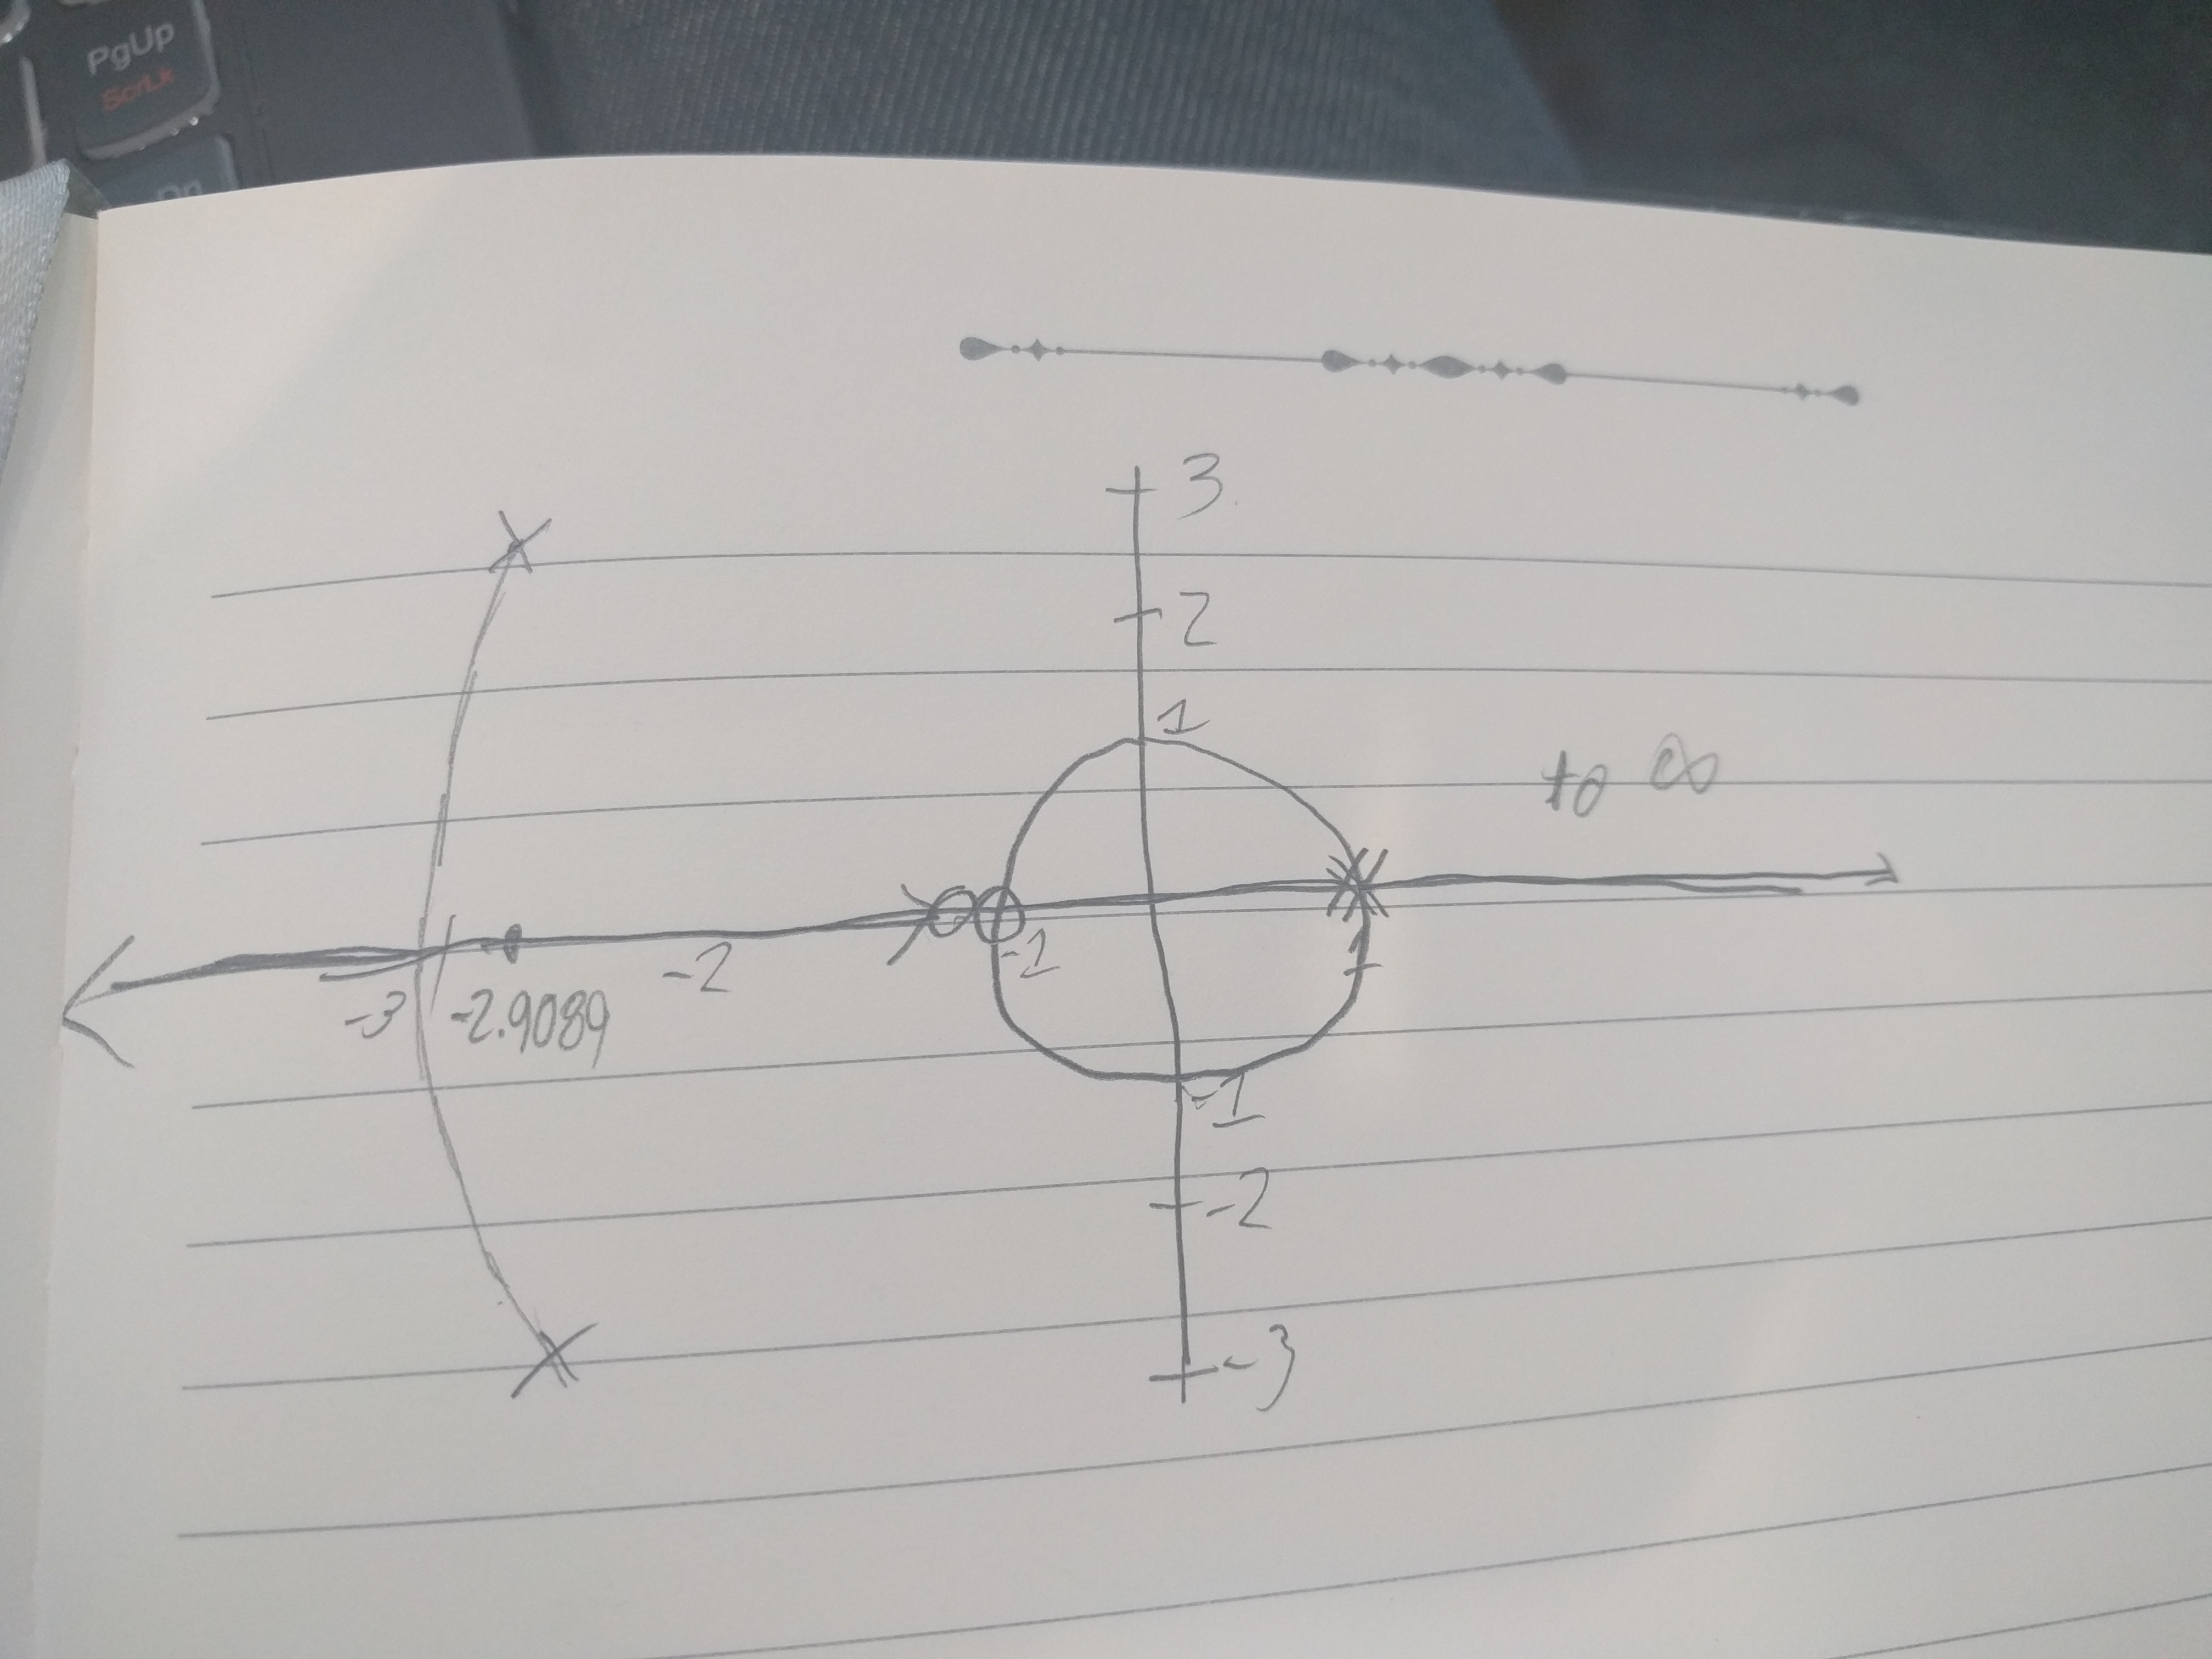
\includegraphics[width=0.7\textwidth]{p2rlocus.jpg}
    \caption{The root locus for the full system described above}
\end{figure}

\subsection*{(e)}
Determine how the system should be changed such that the estimator error isn't effected by the reference input. That is, what are $\pmb{M}$ and $\pmb{N}$. What are the zeros of the overall closed loop system?\\
Begin by finding $\pmb{N}$:
\[\begin{bmatrix}\pmb{N}_x\\\pmb{N}_u\end{bmatrix}=\left (\begin{bmatrix}\pmb{\Phi}-\pmb{I}&\pmb{\Gamma}\\\pmb{H}&0\end{bmatrix}\right)^{-1}\begin{bmatrix}0\\0\\1\end{bmatrix}=\left (\begin{bmatrix}0&0&\frac{1}{21*5}\\0.2&0&\frac{1}{42*25}\\0&1&0\end{bmatrix}\right )^{-1}\begin{bmatrix}0\\0\\1\end{bmatrix}\]
This leads to $N_u=0$ and $N_x=\begin{bmatrix}0\\1\end{bmatrix}$. Which means $N=18.97$ and:
\[\pmb{M}=\begin{bmatrix}\cfrac{18.97}{21*5}\\[0.7em]\cfrac{18.97}{42*25}\end{bmatrix}\]

Given that we picked $M=\Gamma N$ the zeros are:
\[\det\left (\begin{bmatrix}z-1&113\\-0.2&z-1-l2\end{bmatrix}\right )\]
So our zeros are $-2.8\pm 2.8566j$.

\subsection*{(f)}
Suppose that our sensor only measures error and not the state value. That gives $\pmb{M}=-\pmb{L}_p$ and $N=0$. In this case what are the zeros of the closed-loop system? Which of this controller and the one in part e would yield more desirable response?\\
The zeros become:
\[\det(z\pmb{I}-\pmb{\Phi})\pmb{K}(z\pmb{I}-\Phi)^{-1}\pmb{L}_p=0=(z-1)^2\pmb{K}\cfrac{\begin{bmatrix}z-1&0\\-T&z-1\end{bmatrix}}{(z-1)^2}\pmb{L}_p\]
This is:
\[\pmb{K}\begin{bmatrix}113z-113\\7.6z-31.2\end{bmatrix}=20.98*113(z-1)+18.97(7.6z-31.2)=0\]
    Thus we get that the zero is at $1.1780$. The more desirable response would be from the system in part (e). in that case we have more control over the states and a better manipulation of the input.

\subsection*{(g)}
Suppose a current estimator is deemed necessary for better performance. Design $\pmb{L}_c$ such that the error dynamics using the current estimator have the same poles as those designed for the prediction estimator in part (a).\\
We use the fact that $\pmb{L}_c=\pmb{\Phi}^{-1}\pmb{L}_p$:
\[\pmb{\Phi}^{-1}=\begin{bmatrix}1&0\\-0.2&1\end{bmatrix}\]
and we get that:
\[\pmb{L}_c=\begin{bmatrix}113&0\\-22.6&7.6\end{bmatrix}\]

\section*{Problem 3}
Problem 8.11 from the book:
\subsection*{(a)}
Show that the equations for the current estimator can be written in standard state form:
\[\epsilon_{k+1}=\pmb{A}\epsilon_k+\pmb{B}y_k,\quad \pmb{u}_k=\pmb{C}\epsilon_k+Dy_k\]
where $\epsilon_k=\hat{\pmb{x}}_k-\pmb{L}_cy_k$, $\pmb{A}=(\pmb{I}-\pmb{L}_c\pmb{H})(\pmb{\Phi}-\pmb{\Gamma}\pmb{K}),$ $\pmb{B}=\pmb{A}\pmb{L}_c$, $\pmb{C}=-\pmb{K}$, and $D=-\pmb{K}\pmb{L}_c$.\\
We know the current estimator equation is:
\[\bar{\pmb{x}}_{k+1}=\pmb{\Phi}\bar{\pmb{x}}_k+\pmb{\Gamma}\pmb{u}_k+\pmb{\Phi}\pmb{L}_c(y_k-\pmb{H}\bar{\pmb{x}}_k)\]
and the equation relating $\hat{\pmb{x}}_k$ to $\bar{\pmb{x}}_k$
\[\hat{\pmb{x}}_k=\bar{\pmb{x}}_k+\pmb{L}_c(y_k-\pmb{H}\bar{\pmb{x}}_k)\]
Substituting straight in:
\[\begin{split}\epsilon_{k+1}=(\pmb{I}-\pmb{L}_c\pmb{H})(\pmb{\Phi}-\pmb{\Gamma}\pmb{K})(\hat{\pmb{x}}_k-\pmb{L}_cy_k)+(\pmb{I}-\pmb{L}_c\pmb{H})(\pmb{\Phi}-\pmb{\Gamma}\pmb{K})\pmb{L}_cy_k\\
\pmb{u}_k=-\pmb{K}\hat{\pmb{x}}_k\end{split}\]
We can simplify a little bit to:
\[\epsilon_{k+1}=\hat{\pmb{x}}_{k+1}-\pmb{L}_cy_{k+1}=\bar{\pmb{x}}_{k+1}-\pmb{L}_c\pmb{H}\bar{\pmb{x}}_{k+1}=(\pmb{I}-\pmb{L}_c\pmb{H})(\pmb{\Phi}-\pmb{\Gamma}\pmb{K})\hat{\pmb{x}}_k\]
One more subsitution:
\[(\pmb{I}-\pmb{L}_c\pmb{H})\bar{\pmb{x}}_{k+1}=(\pmb{I}-\pmb{L}_c\pmb{H})(\pmb{\Phi}-\pmb{\Gamma}\pmb{K})(\bar{\pmb{x}}_k+\pmb{L}_c(y_k-\pmb{H}\bar{\pmb{x}}_k))\]
simplifying:
\[\bar{\pmb{x}}_{k+1}=\pmb{\Phi}\bar{\pmb{x}}_k-\pmb{\Gamma}\pmb{K}\bar{\pmb{x}}_k+\pmb{\Phi}\pmb{L}_c(y_k-\pmb{H}\bar{\pmb{x}}_k)-\pmb{\Gamma}\pmb{K}\pmb{L}_c(y_k-\pmb{H}\bar{\pmb{x}}_k)\]
One last step:
\[\bar{\pmb{x}}_{k+1}=\pmb{\Phi}\bar{\pmb{x}}_{k}+\pmb{\Gamma}\pmb{u}_k+\pmb{\Phi}\pmb{L}_c(y_k-\pmb{H}\bar{\pmb{x}}_k)\]
Showing that the substitutions are equivalent.
\subsection*{(b)}
Use the results of eq. (4.65) to show that the controller based on a current estimator always has a zero at $z=0$ for any choice of control law $\pmb{K}$ or estimator law $\pmb{L}_e$.\\
Equation 4.65 states that:
\[\begin{bmatrix}z\pmb{I}-\pmb{\Phi}&-\pmb{\Gamma}\\\pmb{H}&0\end{bmatrix}\begin{bmatrix}X(z)\\U(z)\end{bmatrix}=\begin{bmatrix}\pmb{0}\end{bmatrix}\]
For us this equation will change to:
\[\begin{bmatrix}z\pmb{I}-\pmb{\Phi}+\pmb{\Gamma}\pmb{K}+\pmb{L}_c\pmb{H}\pmb{\Phi}-\pmb{L}_c\pmb{H}\pmb{\Gamma}\pmb{K}&-\pmb{L}_c\\-\pmb{K}&0\end{bmatrix}\begin{bmatrix}\hat{X}(z)\\Y(z)\end{bmatrix}=\begin{bmatrix}\pmb{0}\end{bmatrix}\]
Which should give a delay because their is no direct propogation to the output. We can also reduce this by multipling the bottom row by $\pmb{\Gamma}$ from the left and adding that to the top row. Then multiple the right column by $\pmb{H}(\pmb{\Phi}-\pmb{\Gamma}\pmb{K})$ from the right to get:
\[\begin{bmatrix}z\pmb{I}-\pmb{\Phi}&-\pmb{L}_c\\-\pmb{K}&0\end{bmatrix}\]
and using the same analysis as equation 4.65 we get the desired result.
\section*{Problem 4}
Given the double-integrator system:\\
\[x(k+1)=\pmb{\Phi}x(k)+\pmb{\Gamma}u(k),\quad y(k)=\pmb{H}x(k)\]
where:
\[\pmb{\Phi}=\begin{bmatrix}1&T\\0&1\end{bmatrix},\quad \pmb{\Gamma}=\begin{bmatrix}\cfrac{T^2}{2}\\T\end{bmatrix},\quad \pmb{H}=\begin{bmatrix}1&0\end{bmatrix}\]
where $T$ is the sample period.
\subsection*{(a)}
Design a reduced-order estimator gain vector $\pmb{L}_r$ such that the reduced-order estimator pole is $\alpha$. How does $\pmb{L}_r$ change as the magnitude of teh estimator pole $\lvert\alpha\rvert$ becomes smaller (i.e., faster pole)? Consider $\alpha >0$ and $\alpha <0$ separately.\\
We get that:
\[x_2(k+1)=x_2(k)+Tu(k)\]
and:
\[x_1(k+1)-x_1(k)-\cfrac{T^2}{2}u(k)=Tx_2(k)\]
We can then move the pole:
\[z-\alpha=\det(z-(1-L_rT))=0\]
and thus $L_r=\frac{1-\alpha}{T}$. Smaller $\alpha$ values for positive $\alpha$ make value of $L_r$ converge to $\frac{1}{T}$ from negative infinity. Negative alpha will converge from the other side at positive infinity to $\frac{1}{T}$.
\subsection*{(b)}
Suppose that the sensor has a small constant offset, so that
\[y(k)=\begin{bmatrix}1&0\end{bmatrix}\pmb{x}(k)+0.01\]
How does this affect the estimate of $x_2(k)$ using the reduced-order estimator you designed in part(a)? Does the estimate of $x_2(k)$ have an offset as well? If so, find an expression for this offset on $\hat{x}_2$. If not, explain why.\\
Just looking at:
\[\hat{x}_b(k+1)=\Phi_{bb}\hat{x}_b(k)+\Phi_{ba}x_a(k)+\Gamma_bu(k)+L_{rp}(x_a(k+1)-\Phi_{aa}x_a(k)-\Gamma_au(k)-\Phi_{ab}\hat{x}_b(k)\]
Thus the extra term will propogate through $\Phi_{ba}x_a(k)$ and the added offset will be $\Phi_{ba}*0.01$.

\end{document}
